\documentclass[12pt, titlepage]{article}
\usepackage[utf8]{inputenc}
\usepackage[hidelinks]{hyperref}
\usepackage{graphicx}

\renewcommand{\contentsname}{Innehållsförteckning}


\begin{document}
\title{
  Marinmuseum på ett interaktivt sätt!\\
  (Grupp 17, 2015)\\
%  \vspace{0.2in}
}

\author{
  Alex Hoeing\\
  \url{alex.l.hoeing@gmail.com}\\
  Liam Wolter\\
  \url{Liamwolter@live.se}\\
  Albin Hammarström\\
  \url{Albin.hammarstrom95@gmail.com}\\
  Erik Bihl\\
  \url{Eribih@gmail.com}\\
}

\date {}


\maketitle

\tableofcontents
\setcounter{page}{0}
\newpage
\section{Introduktion}
\subsection{Inledning}
Vårt projekt består av en webbapplikation som ska hjälpa marinmuseet i Karlskrona att underhålla 
barn med åldern 6-12 år vid plats på marinmuseets magasin, och även underlätta sökning på objekt 
som finns att titta på. Vår idé gick ut på att skapa en slags skattjakt där barnen får 
leta upp QR-koder o sedan få någon slags belöning efter de har skannat de olika objekten som 
vi slumpar ut utifrån ett tema.

\subsection{Bakgrund}
Vid kursstart så skulle vi, studenterna, ta initiativ och välja ut en tredje part 
som vi skulle vilja jobba emot. Skolan hade självklart ett par företag man kunde 
få välja emellan men det gick även bra att på egen hand skapa kontakt med 
ett företag och jobba emot det om så skulle önskas och förutsatt att man kunde göra 
det på egen hand. Vi valde att prova att ta kontakt med ett företag som heter Appcorn, 
och Appcorn är ett företag som utvecklar mobilapplikationer och som har jobbat med stora 
företag så som Coop, Findus och Spotify etc.
\\
\\
Vi mailade företaget och fick till svar att vi kunde komma på ett möte, 
vi antog att de var intresserade utav oss och faktiskt ville ingå i något sorts arbete. 

När vi ankom till Appcorn vid tidspunkten då mötet skulle ta plats blev vi hänvisade 
in i ett grupprum där vi satt ner och fick prata med chefen Mårten Nilsson, 
i detta mötet blev det ingenting av utan de hade inte tid att ingå i något samarbete, 
vilket vi ansåg trist. Så vi fick helt enkelt leta vidare, tre veckor in i kursen kom vi 
i kontakt med Johan Löfgren på Marinmuseum där vi sedan kunde ingå i ett samarbete. 
Målet med vårt arbete och vår produktion var att vi skulle skapa någonting som skulle kunna 
få barn mellan sex och tolv år att kunna tycka att saker som marinmuseum innehaver kan vara 
roligt och att själva upplevelsen är rolig medans man lär sig något.

\section{Projekt titel}
\subsection{Förproduktion}
Från våra projekt tidigare har vi använt oss av några begrepp som har varit väldigt 
användbara till produktionsutvecklingen och förproduktion. Accountability är ett av 
dessa begrepp som vi använt oss av i förproduktionen. 

Vår förproduktion bestod av att 
vi till en början gjorde klart för oss vad som skulle göras innan vi började planera hur vi skulle jobba. 
För att kunna säkerställa att det vi kom fram till var en önskvärd idé så har vi haft öppen kommunikation med Marinmuseum. 
När vi hade fastställt idén så var det egentligen bara att sätta igång, 
att börja planera allting från vad vi skulle använda för verktyg till planering av tid och deadlines. 
Därefter gick vi igenom vilka risker det fanns med projektet, vad som kunde gå fel. 

Vi i gruppen pratade mycket om hur vi skulle hantera objekt t.ex. vapen och sen göra det barnvänligt. 
Vi var även tvungna att tänka på hur ljudet till objekten skulle vara t.ex. skulle vi har 
ett ljud på när en kanon skjuts eller är det något som inte passar barn som är mellan 6 till 12 år. 
De som är 12 år kanske tycker det är häftigt medans någon som är 6 år tycker det är läskigt. 
Skillnaden mellan någon som är 6 och någon som är 12 är väldigt stor, vilket gjorde lite mer utmanande än vad vi hade tänkt oss.
\begin{center}
  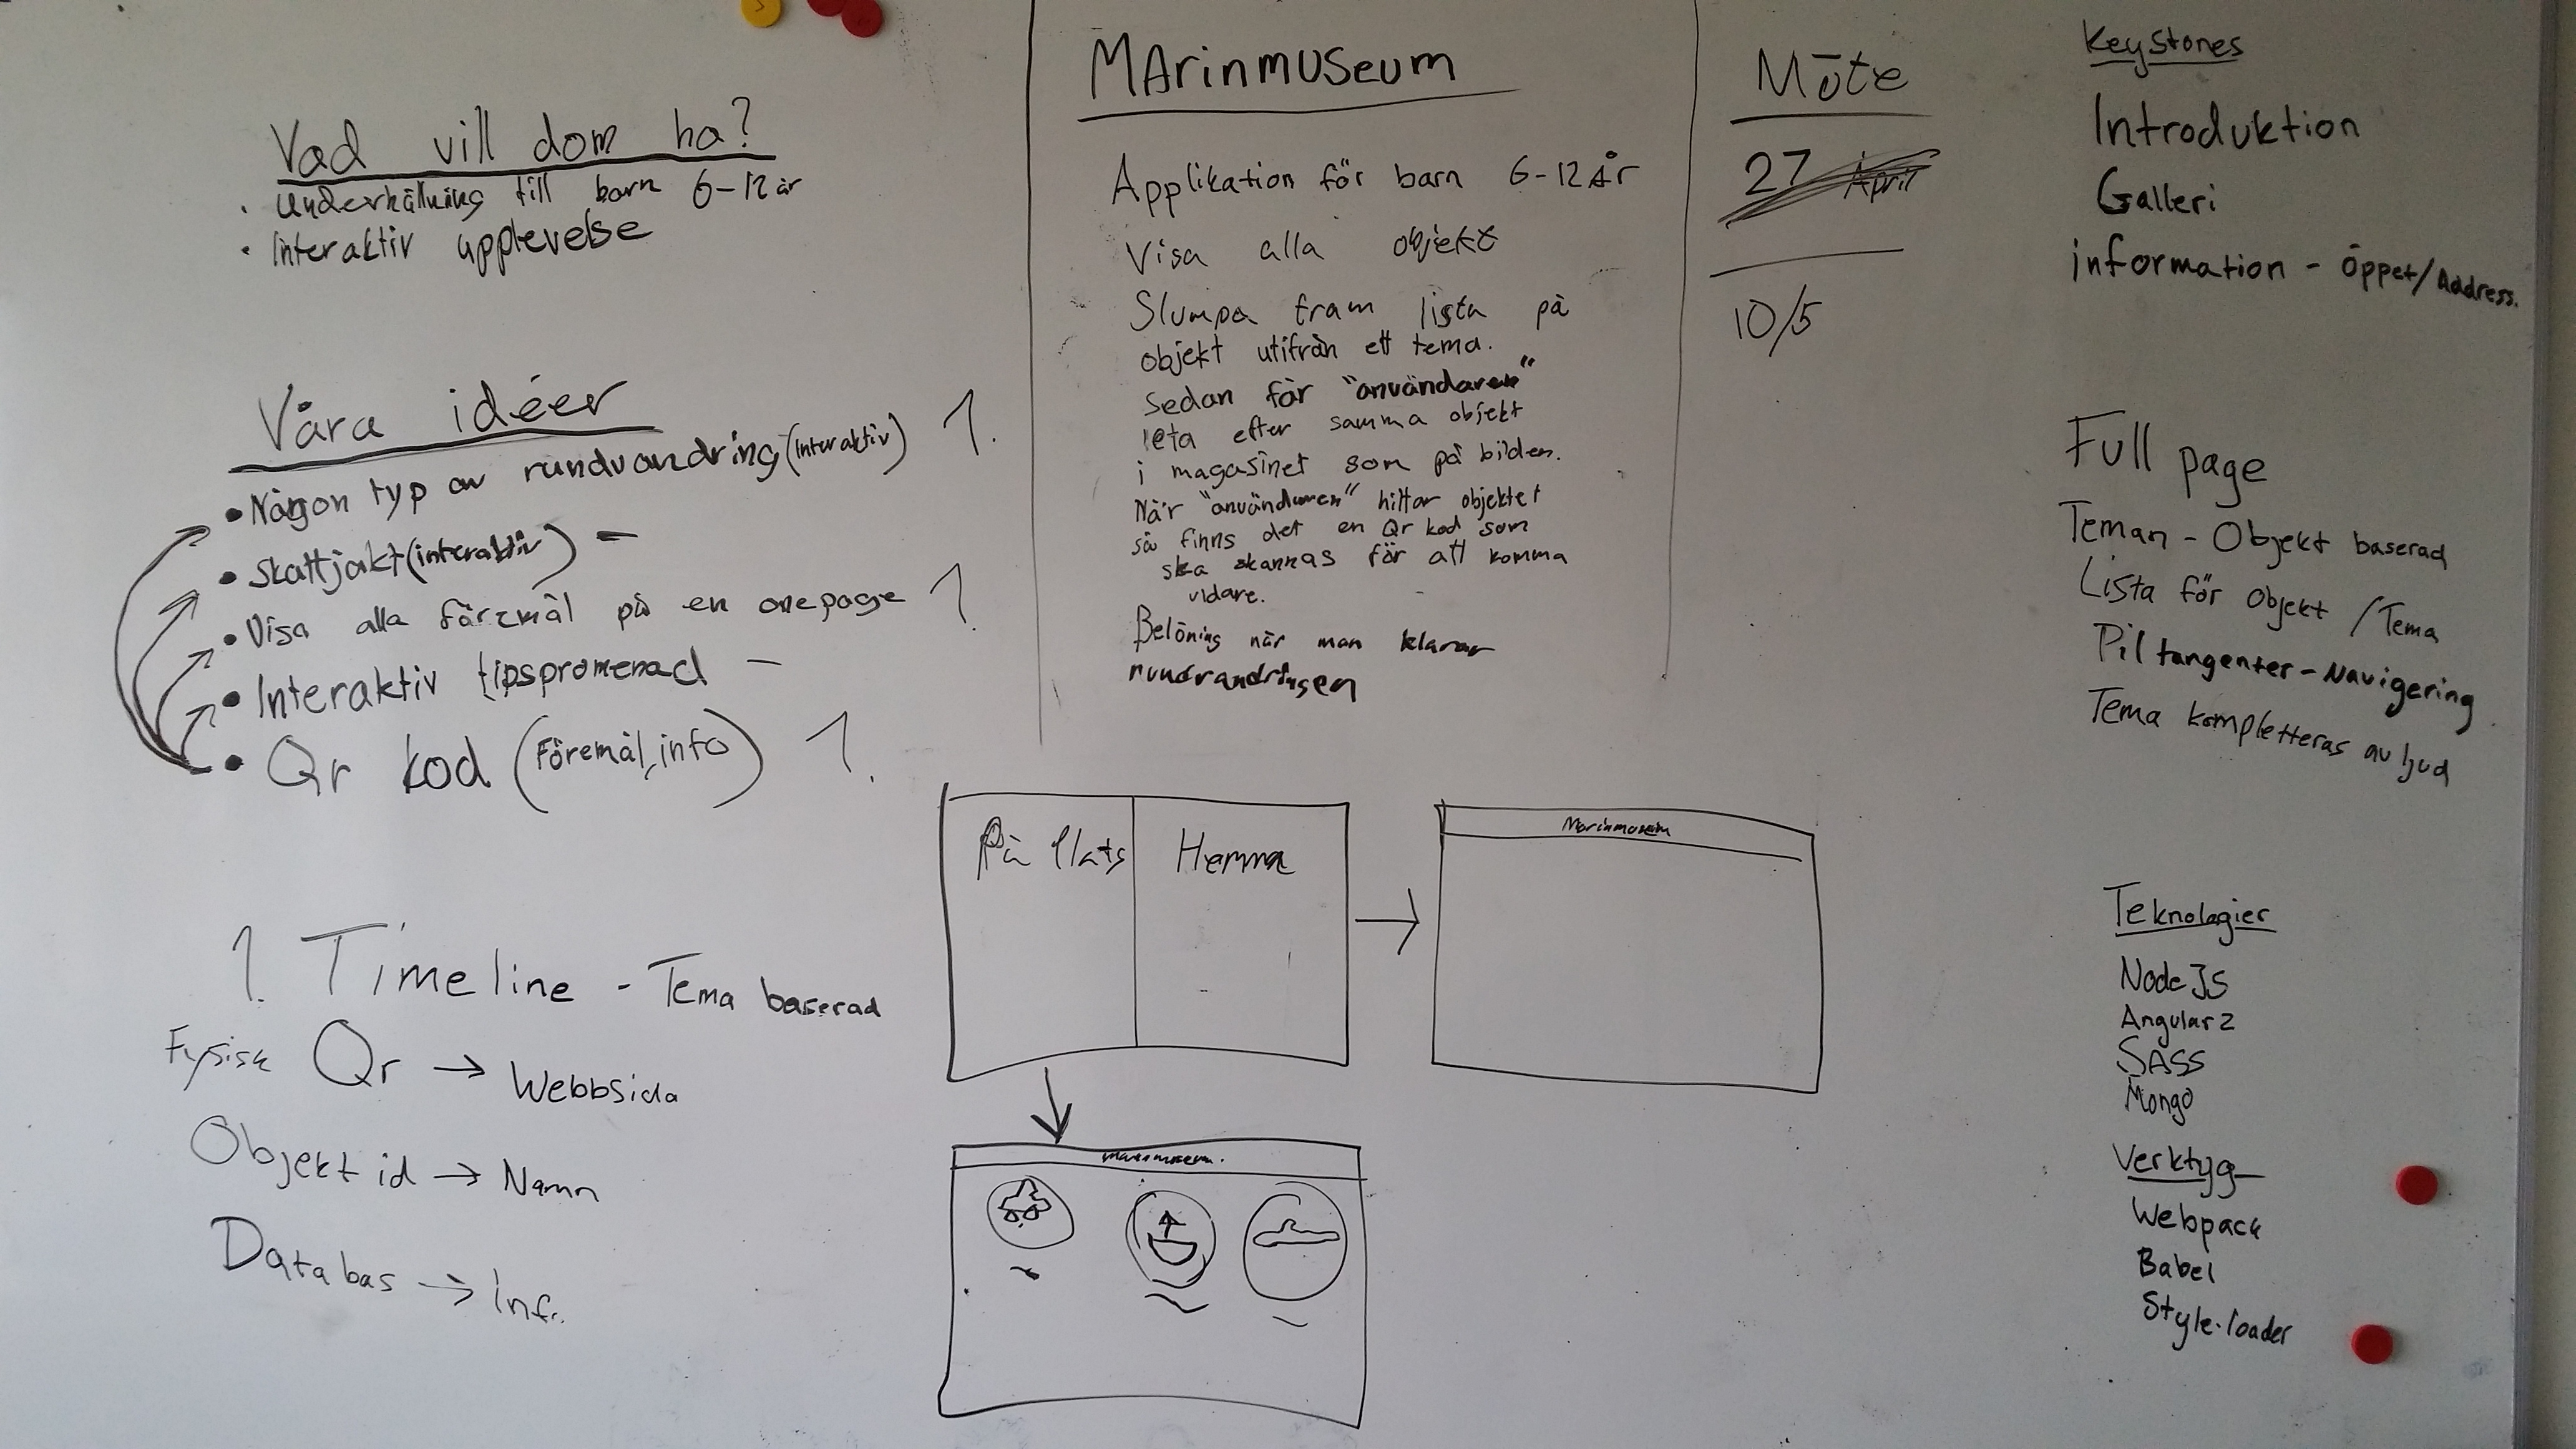
\includegraphics[width=1.0\textwidth]{tavla}
\end{center}
\begin{center}
Bilden ovan visar vad vi kom fram till. 
\end{center}
\newpage
På höger sida skrev vi vad marinmusuem ville ha, samt står det vad vi kom 
fram till utifrån deras krav. I mitten ser man vår ursprungliga design av webbapplikationen, vilket senare ändrades. 
På vänster sida står det vilka teknologier och verktyg vi tänkte använda. 
\\
Följande punkter var kritiska i planeringen:
\begin{enumerate}
  \item Environment (Verktyg \& Teknologier)
  \item Tid (Upplägg av vår tid)
  \item Design av applikationen
  \item Design av infrastrukturen
\end{enumerate}
När dessa punkter var väl strukturerade och godkända enligt vår egen bedömning så kunde vi påbörja produktionen av applikation.

\subsection{Produktion}
Produktionen startade inte förrän ungefär 3-4 veckor in i kursen, allt började med att vi hade tänk oss
vända oss till ett annat företag men de backade ur ungefär 2 veckor efter kursstart, 
så vi försökte då vända oss till marinmuseet där vi hade svårt att ta kontakt till en början.	
Förproduktionen tog upp ungefär två veckor där vi ständigt diskuterade vad som var rätt för oss och vad som i
sin tur skulle vara lätt för kunden att hantera efteråt, efter förproduktionen påbörjade vi då vår produktion. 

Vi kom fram till vad vi anser en utmärkt idé tillsammans med Marinmuseum, vi valde att skapa en webbapplikation 
som ska kunna fungera som en “extention” till museet på plats. Applikationen har två huvudfunktioner som utfyller applikationens syfte. 
Den ska både funka som ett sorts online magasin där du fritt kan bläddra mellan de olika objekten som finns i 
museet men den ska också funka som en anslutning för barn till museet. Vårt svar på detta var att skapa en skattjakt som barnen 
kan interagera med genom en surf-platta och på så sätt göra upplevelsen roligare och förhoppningsvis mer lärorik.
\\
\\
Även om vi har en tanke om hur applikationen ska se ut vid slutet av kursen så blir den aldrig riktigt klar ändå, 
det finns alltid plats för förändring och nya funktioner, kanske till och med plats för omskrivning av koden och 
borttagning av vissa funktioner.

Löwgren (2004) säger “Produkten blir egentligen aldrig färdig, 
utan den förändras under hela sin livstid genom användarnas egen försorg eller genom att designern 
gör nödvändiga åtgärder baserade på långsiktiga fältstudier”(s.119). 

Detta är något vi alla i gruppen kan relatera till, 
att även om man har en tydlig bild tillsammans eller individuellt så blir resultatet oftast inte det man har tänkt 
sig utan oftast lägger man till nya saker för att man inser att man behöver ny eller mer funktionalitet, 
eller så tar man bort saker för att man inser att funktionaliteten inte behövs längre.
\\
\\
Även om man lägger till eller tar bort funktioner, design eller annat som relaterar till applikationen, 
så måste det inte innebära att applikationen i sig är dålig, om man spenderar mer tid i en produktion 
så får man kontext och man börjar förstå och inse saker som man trodde sig veta men som man i realiteten inte 
riktigt hade kunnat tänka sig. Detta är bra för att oavsett hur du utvecklar din produktion så kan det endast går framåt, 
även om man gör val som anses mindre bra så kommer det antagligen reda ut sig under produktionens gång då 
applikationen aldrig blir klar utan endast kan på byggas till något nytt.

\section{Avslutningsvis}
\subsection{Slutsats}

\subsection{Reflektion}
Något vi gemensamt har fått känna av är att produktionen i sig kändes påskyndat i och med vi började lite sent, 
i vår åsikt. Vi hade hellre velat starta förproduktionen sedan dag ett istället för att ha påbörjat den tre veckor senare. 
Dock så betyder det inte att den allmänna upplevelsen för oss som utvecklar applikationen är dålig, 
utan Johan och Louise har varit bekväma att jobba med. De är alltid bara ett mail iväg. 

Vi hade dock velat att de var mer aktiva i vårt projekt. Det kändes lite som att de inte villa vara delaktiga utan låta 
oss komma fram till målet själva, medans vi förväntade oss att de skulle ge mycket feedback och komma fram 
med idéer på hur det skulle kunna implementeras i deras nuvarande situation. 

En anledning till att de inte var aktiva deltagande 
kan beror på att skolan sa till dem att vi elever skulle komma fram med förslag till att lösa externa partners problem. 
Detta är inget något negativt, men jag tror marinmuseum och kanske några andra partners trodde då att de skulle 
håla sig borta och låta oss elever ta hand om problemet själva, medans de observerar över processen. 

Något som kanske skulle behöva förtydligas är att efter eleverna har kommit fram till en idéer, 
så kan de externa parters ge feedback om idén och sen komma fram till något som passar båda grupperna. 
En annan anledning till att de inte var aktivt deltagande kan bero på att inga pengar var involverade och 
de kanske kände att det skulle vara orättvist för oss om de började försöka få in oss på något annat spår.
\\
\\
Även uppgiften har varit väldigt intressant i vår åsikt, vi har fått testa på att utveckla någonting som skulle 
tilltala barnen och samtidigt hålla en stark knytning till objekten som finns på det marinmuseum. 
Tidigare har inte vi försökt rikta oss in på barnen och därför var detta något helt nytt och roligt.
\\
\\
Nu får vi det att låta som att våra känslor kring projektet har varit blandade då vi antyder att vi 
har varit stressade men samtidigt har älskat produktionen vid varje steg av utvecklingen och det är ungefär det vi försöker få fram. 

Vi har haft hinder, vissa svårare än andra. Men det är det som gör utvecklingen av en produkt intressant och får 
producenten att vilja fortsätta i våra ögon. Det har helt enkelt varit en otroligt rolig och 
stressig produktion vi har fått involvera oss i och vi har tyckt om det hela vägen.
\end{document}
